\documentclass{article}
\usepackage{minted}
\usepackage{listings}
\usepackage{csvsimple}
\usepackage{graphicx}
\usepackage{supertabular}
\usepackage{multicol}
\usepackage[section]{placeins}

\graphicspath{{../figures/}}

\title{AMATH 582 Homework 1: A submarine problem}
\author{Brady Griffith}
\date{January 27, 2021}

\begin{document}
    \maketitle

    \begin{abstract}
        In this project, 49 wide spectrum sonar recordings are used to identify that a submarine in the Pudget Sound with a characteristic frequency around $k_x=-0.078$, $k_y=-0.125$, and $k_z = 0.047$. When filtering out other noise at other frequencies, the location of the submarine in each recording becomes observable. The location is automatically detected to give a the submarine's path.
    \end{abstract}

    \section{Introduction and Overview}
    The data set presented for this problem contains 49 spectrum acoustic measurements over a 24 hour period. These should contain the signature of a submarine, but the noise is too high. Since the submarine is moving, it isn't possible to simply average all of the samples.

    Instead, it would be preferable to remove as much of the noise as possible without changing the submarine information. If the submarine produces a characteristic frequency, a band pass filter around it would remove most of the noise while leaving the signal intact.

    The objective of this project is to first determine the frequency signature of the submarine. Then, with filtering, determine the submarine's location in each recording. Finally, the x-y coordinates of the submarine need to be reported so that a P-8 Orion may be deployed to follow the submarine.
    
    This process was modeled in a single dimension in both the textbook for this course \cite{kutz_2013} and the lectures. This project applies that methodology, but now in 3D. It also asks for a more quantitative statement about the location of the submarine, so an automated process to identify the peak in space is developed.

    \section{Theoretical Background}
    The key principle allowing this analysis has to do with how a shift in space affects the wavenumber, and vice versa. As an illustration of this point, consider the following signal in space
    \begin{equation}
        f(x) = A e^{2 \pi i k_0 x} \frac{1}{\sigma \sqrt{2 \pi}} e^{\frac{-(x-x_0)^2}{2 \sigma^2}}
    \end{equation}
    and its fourier transform
    \begin{equation}
        \hat{f}(k) = A e^{-2 \pi i (k - k_0) x} e^{\frac{-(k - k_0)^2 \sigma^2}{2}}
    \end{equation}
    The important observation is that when moving the submarine in time (by shifting $k_0$), it only affects the complex phase of the fourier transform, not the magnitude. This means that, as long as the center frequency remains the same, the movement of the submarine will not affect the power spectral density.

    When examining the signal in frequency space, I make use of the power spectral density (PSD). It is defined as follows
    \begin{equation}
        PSD(k_x, k_y, k_z) = \frac{1}{2} \frac{|\hat{f}(k_x, k_y, k_z)|^2}{(\Delta k)^3}
    \end{equation}
    where $\hat{f}(k_x, k_y, k_z)$ is the fourier transform of the signal. It has the advantage of being real and positive. It also has reasonable physical intuition, as integrating the PSD over some volume of frequency space gives the energy there. The unspecified units of this problem however mean that this is much less important.

    \section{Algorithm Implementation and Development}
    The data is loaded from the \lstinline{subdata.mat} file using the scipy \lstinline{scioy.io.loadmat} function. The axes that will be used with the signal in both time and frequency space are calculated. Note that when calculating the wavenumber using \lstinline{np.fft.fftfreq}, you must multiply by (2*np.pi/(2*L)) so that it is scaled correctly to angular frequency.
    
    The discrete fourier transform of the provided recordings is calculated using the numpy n dimentional fft, \lstinline{numpy.fft.fftn}. This is then averaged over all of the recordings and then the PSD of this is calculated. It is projected onto the x-y, x-z, and y-z axes so that the shape of the characteristic frequency can be noted and used when deciding filter parameters.

    The frequency response along each axis, integrating the perpendicular PSD, yields the total energy per slice width of that axis. The advantage of looking at it this way is that finding the peak now becomes a 1D problem. The result is a smooth bell curve shaped peak around the center frequency. I would like to identify two properties of this, the location of the center and it's width, so the filer can sufficiently wide.

    I choose to find this by fitting the $k_{0i}$, $bg$, $\sigma$, and $A$ parameters in equation \ref{eq:model_f} using the scipy \lstinline{scipy.optimize.curve_fit} function. This projection along with the best fit is illustrated in figure \ref{fig:axes_fit}. This has the advantage of being simple to implement and tolerant of the remaining noise. This sort of optimization is well behaved on this data, so I don't need to worry about common problems like false fits. It does have the disadvantage of being slow, but since this is only used a few times on this problem, I am willing to accept the added computation time for the simplicity. This was used instead of manually determining the parameters because this code could be reused when identifying the submarine position.

    \begin{equation} \label{eq:model_f}
        f(k_i) = \frac{A}{\sqrt{2 \pi} \sigma} \exp{-\frac{(k_i - k_{i0})^2}{2 \sigma}} + bg
    \end{equation}

    \begin{figure} \label{fig:axes_fit}
        \centering
        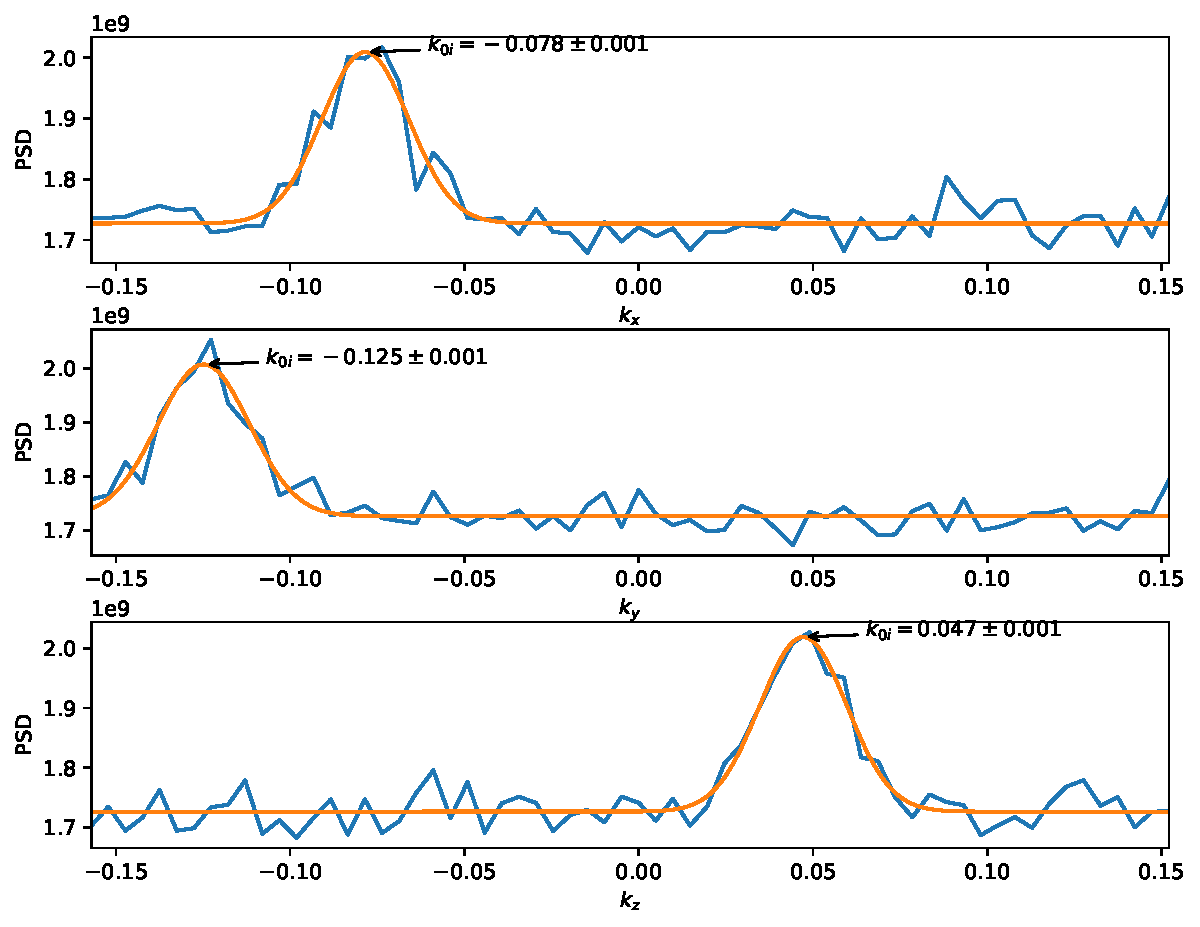
\includegraphics[width=\textwidth]{axes_fit.pdf}
        \caption{The PSD of the frequency averaged over all recordings, projected onto the 3 axes, along with the best fit curve in orange.}
    \end{figure}

    
    In order to get the best results some care must be taken that the initial value of the optimization are somewhat close to solution. As such, I chose the initial background, $bg$, to be the minimum of the data. I chose $A$ to be the integral over the axis of the data with $bg$ subtracted. I chose $k_{0i}=0$, the center of the range and $w=8 \Delta k$, $1/8$ of the axis.

    With the central frequency characterized, it is time to multiply a filter to remove the noise away from it. A gaussian filter is used because a sharp cutoff is not needed, but the introduction of any ringing into the space domain would be unideal. The filter used was a symmetric 3D gaussian about some center $(k_{0x}, k_{0y}, k_{0z})$

    \begin{equation}
        \mathcal{F}(k_x, k_y, k_z) = \frac{1}{(2 \pi \sigma^2)^{3/2}} \exp \left( -\frac{(k_x - k_{0x})^2 + (k_y - k_{0y})^2 + (k_z - k_{0z})^2}{2 \sigma^2} \right)
    \end{equation}

    This is a simple design for the filter. A true 3D gaussian with 3 different covariance axes might have been able to reduce the noise further while preserving the signal, but this design is good enough to leave the a prominent maximum, and much simpler to determine the ideal parameters.

    The width is chosen to be the center of the fits to equation \ref{eq:model_f}. The width, $\sigma$, is chosen to be twice the maximum of the axes' fit for standard deviations. This is multiplied and then the inverse discrete fourier transform ia taken, again using the function from numpy. This then results in 49 different 3D recordings with a prominent peak.

    The same fitting functions are then used again. Here it is used 49 times, far too many to manually identify each peak, but still few enough to not seek a computationally efficient peak identifier. The center from each best fit reported and then put in a list to plot the path.

    \section{Computational Results}
    The submarine produces a characteristic frequency centered at $k_x=-0.078$, $k_y=-0.125$, and $k_z = 0.047$. It's shape is shown projected in figure \ref{fig:freq_proj}. It appears to flattened along the $\left< 1, -1, 0 \right>$.

    \begin{figure} \label{fig:freq_proj}
        \centering
        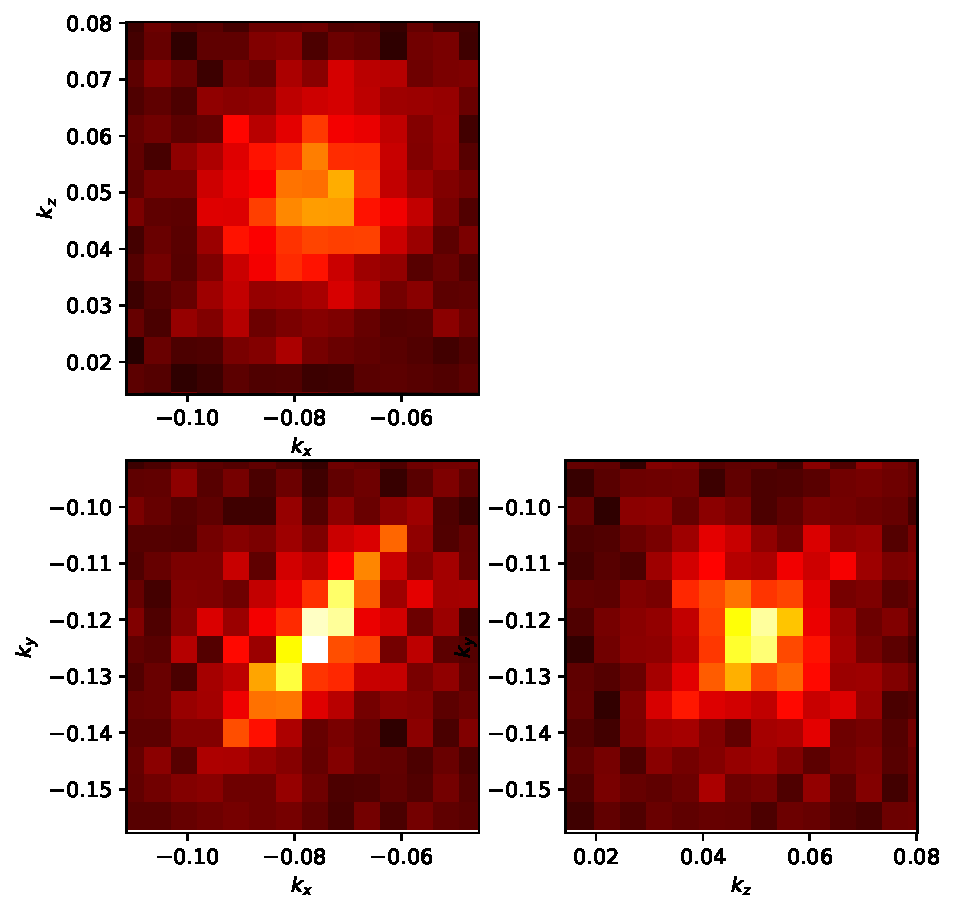
\includegraphics[width=.8\textwidth]{projected_freq.pdf}
        \caption{Total PSD of the frequency averaged over all recordings, integrated along the perpendicular axis for the x-y, y-z, and x-z planes. This shows the shape of submarine's characteristic frequency.}
    \end{figure}    

    The submarine travels from $(3.017,-7.984,-0.012)$ to $(-5.093,6.423,0.840)$. The full path is drawn in figure \ref{fig:path}.

    \begin{figure} \label{fig:path}
        \centering
        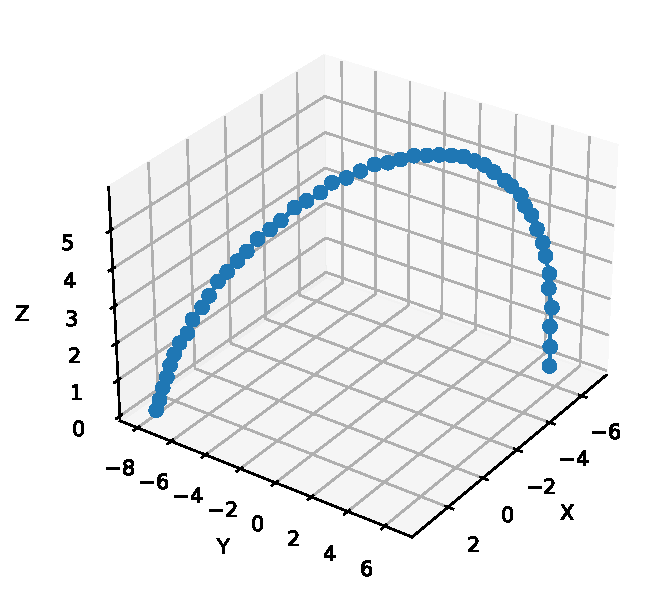
\includegraphics[width=.6\textwidth]{path.pdf}
        \caption{Path of the submarine. Each dot is the location during one of recordings. You can see the movement of the sub in half hour steps.}
    \end{figure}

    % \newpage
    % \begin{figure}
    %     \footnotesize	
    %     \begin{multicols*}{2}
    %         \tablehead{\hline & \textbf{X} & \textbf{Y} & \textbf{Z} \\ \hline}
    %         \tabletail{\hline}
    %         \begin{supertabular}{|l|l|l|l|}
    %         \csvreader[%
    %             late after line=\\]%
    %             {../figures/position.csv}{1=\x,2=\y,3=\z}%
    %             {\thecsvrow & \x & \y & \z}
    %         \end{supertabular}
    %     \end{multicols*}

    %     \caption{Table of positions}
    % \end{figure}

    \section{Summary and Conclusions}
    When filtered to just the characteristic frequency of the submarine, $k_x=-0.078$, $k_y=-0.125$, and $k_z = 0.047$, the location can clearly be picked out in each recording. The submarine ends at the XY position $(-5.093, 6.423)$. I would send the P-8 Orion there so it can follow the submarine.

    \bibliographystyle{ieeetr}
    \bibliography{bibliography}

    \FloatBarrier
    \newpage
    \appendix
    \section{Python Functions}
        I'm going to leave out this section in the future, since it seems redundant. For the information that would be here, I direct the reader to the docstrings at the beginning of each function.

    \section{Python Code}

    \subsection{main.py}
    \inputminted{python}{../code/main.py}

    \subsection{fourier.py}
    \inputminted{python}{../code/fourier.py}

    \subsection{peakfinding.py}
    \inputminted{python}{../code/peak_finding.py}

    \subsection{visualize.py}
    \inputminted{python}{../code/visualize.py}

\end{document}